\documentclass[a4paper, 12pt, titlepage]{article}

% Including needed packages
\usepackage[margin=2cm]{geometry}
\usepackage{amsmath}
\usepackage{amssymb}
\usepackage{amsthm}
\usepackage{graphicx}
\usepackage{subfig}
\usepackage{float}
\usepackage{pgf}
\usepackage{tikz}
\usepackage{dsfont}

\newcommand{\norm}[1]{\lVert#1\rVert}
\usetikzlibrary{automata,positioning}

\title
{{\em Machine learning 2}\\
Exercise sheet 9}
\author{FLEISCHMANN Kay, Matrnr: 352247\\
	ROHRMANN Till, Matrnr: 343756}
\date{\today}

\begin{document}

\maketitle

\section{Hidden Markov Models}
Let $A_{i,j}$ the transition matrix between hidden states $x_i$ and $x_j$. $B_{i,j}$ is the the probability, beeing in state $x_i$ to observe $y_j$.
The following matrices $A$ and $B$ describe two hidden states and two possible observations.

\[
A= 
 \begin{pmatrix}
  0.1 & 0.9 \\
  0.5 & 0.5
 \end{pmatrix}
\]

\[
B=
 \begin{pmatrix}
  0.2 & 0.8 \\
  0.4 & 0.6
 \end{pmatrix}
\]

\subsection*{a. Draw the graph of the model}
The Hidden-Markov-chain for $A$ and $B$ looks like the following4

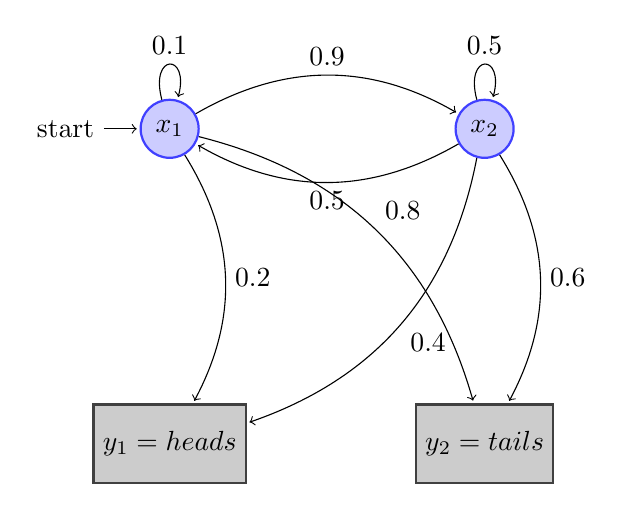
\begin{tikzpicture}[shorten >=1pt,node distance=2cm,on grid,auto] 
  \tikzstyle{state}=[circle,thick,draw=blue!75,fill=blue!20,minimum size=6mm]
  \tikzstyle{observation}=[rectangle,thick,draw=black!75,
  			  fill=black!20,minimum size=10mm]
  			  
  \node[state,initial] (x1)   {$x_1$};
  \node[state] (x2) [right=4cm of x1] {$x_2$};
  \node[observation] (y1) [below=4cm of x1] {$y_1=heads$};
  \node[observation] (y2) [right=4cm of y1] {$y_2=tails$};

  \path[->] (x1) edge [bend left] node {0.9} (x2);
  \path[->] (x2) edge [bend left] node {0.5} (x1);
  \path[->] (x1) edge [loop above] node {0.1} (x1);
  \path[->] (x2) edge [loop above] node {0.5} (x2);

  \path[->] (x1) edge [bend left] node {0.2} (y1);
  \path[->] (x1) edge [bend left] node {0.8} (y2);

  \path[->] (x2) edge [bend left] node {0.4} (y1);
  \path[->] (x2) edge [bend left] node {0.6} (y2);
\end{tikzpicture}
  
Because of $\pi = (1 | 0)$ all state-sequences start with the initial state $x_1$.
  
\subsection*{b.}


\textit{We interpret the above as a model for an experiment with two hidden (unfair) coins and two visible coins. Describe such an experiment which can be modelled by the Markov model given above. Here, heads should correspond to the first indices in $A$, $B$, $\pi$, heads to the second.} \newline \newline

A guy is standing behind an curtain and is throwing two unfair coins, just one each time but starts always with the first one. A second guy in front of the curtain just get the information about the observed heads or tails as a sequence. The task of the second guy is to find the most likely sequence of the thrown coins.


\subsection*{c.}

Given the bayes rule:
\begin{equation}
   P(X|Y(1)=tails,Y(2)=tails) =  \frac{P(Y(1)=tails,Y(2)=tails|X)P(X)}{P(Y(1)=tails,Y(2)=tails)}
\end{equation}

Because of the statistical independence, we can write
\begin{eqnarray}
  P(Y(1),Y(2)|X(1),X(2)) &=& P(Y(1)|X(1)) \cdot P(Y(2)|X(2))
\end{eqnarray}

Furthermore we have
\begin{eqnarray}
	P(X(1)=x_i,X(2)=x_j)&=& P(X(2)=x_j\mid X(1)=x_i) \cdot P(X(1) = x_i) \\
	&=& B_{i,j} \cdot \pi_i
\end{eqnarray}

All possible sequences with length $2$ are

\begin{tabular}{l*{3}{c}r}
              & State sequence & $P(X)$ & $P(Y(1)=tails,Y(2)=tails|X) $ \\
\hline
1 &  $x_1 \rightarrow x_1$ & $P(X(1)=x_1,X(2)=x_1)=0.1$ & $ 0.8\cdot 0.8=0.64 $\\
2 &  $x_1 \rightarrow x_2$ & $P(X(1)=x_1,X(2)=x_2)=0.9$ & $ 0.8\cdot 0.6= 0.48 $ \\
3 &  $x_2 \rightarrow x_1$ & $P(X(1)=x_2,X(2)=x_1)= 0$ & $ 0.6 \cdot 0.8 = 0.48 $ \\
4 &  $x_2 \rightarrow x_2$ & $P(X(1)=x_2,X(2)=x_2)= 0$ & $ 0.6 \cdot 0.6 = 0.36 $
 \end{tabular}

\begin{align}
  P(Y(1)=y_2,Y(2)=y_2) &= \sum_{X \in S^2} P(Y(1)=y_2,Y(2)=y_2|X) P(X)  \\
	     &= \sum_{X \in S^2} P(Y(1)=y_2,Y(2)=y_2|X) P(X) \\
	     &= 0.64\cdot 0.1 + 0.48\cdot 0.9 + 0.48 \cdot 0 + 0.36\cdot 0 \\
	     &= 0.496
\end{align}

The result for $P(X \mid Y(1)=tails,Y(2)=tails)$ follows as

\begin{tabular}{l*{2}{c}r}
              & State sequence &  $P(X|Y(1)=tails,Y(2)=tails)$ & \\
\hline
& & & \\
1 & $X=X(1)=x_1,X(2)=x_1$ & $\frac{0.64 \cdot 0.1}{0.496} \approx 0.129$ \\
& & & \\
2 & $X=X(1)=x_1,X(2)=x_2$ & $\frac{0.48 \cdot 0.9}{0.496} \approx 0.871$ \\
& & & \\
3 & $X=X(1)=x_2,X(2)=x_1$ & $\frac{0.48\cdot 0}{0.496} = 0$ \\
& & & \\
4 & $X=X(1)=x_2,X(2)=x_2$ & $\frac{0.36 \cdot 0}{0.496} = 0$ 
 \end{tabular}

 
\subsection*{f.}
Prove in the scenario of $(e)$ and the assumptions of the exercise: if $N \rightarrow \infty$, then the sample observation frequency of heads/tails at fixed position $n$ converges, in probability and entry-wise, to the vector $\pi \cdot A^n \cdot B$.

\begin{proof}

Given an initial distribution, the probability that we see heads in the sequence of observations $Y$ at position $k$ is $\Pr(Y(k)=y_1)=(\pi \cdot A^k \cdot B)_1$.
Thus we see tails at the position $k$ with probability $\Pr(Y(k)=y_2)=(\pi \cdot A^k \cdot B)_2 = 1- (\pi \cdot A^k \cdot B)_1$.

Running $N$ times the experiment with the same initial distribution, we obtain $Y_i$ observation sequences with $1\le i \le N$.
It holds that for all time points $t$ the observations $Y_i(t)$ of the different run of the experiment are conditonally independent.
In order to calculate the observations frequency of heads we calculate for each position $k$ with $1\le k \le n$ the empirical frequency:

\begin{eqnarray}
	heads_{emp}(k) &=& \frac{1}{N}\sum_{i=1}^N \mathds{1}_{Y_i(k)=y_1} \label{eq:heads}
\end{eqnarray}

The term $\mathds{1}_{Y_i(k)=y_1}$ can be considered a Bernoulli variable whose probability to be $1$ is
\begin{eqnarray*}
	\Pr(\mathds{1}_{Y_i(k)=y_1}=1) &=& (\pi \cdot A^k \cdot B)_1
\end{eqnarray*}
and its probability to be $0$ is
\begin{eqnarray*}
	\Pr(\mathds{1}_{Y_i(k)=y_1}=0) &=& 1-(\pi \cdot A^k \cdot B)_1\\
	&=& (\pi \cdot A^k \cdot B)_2
\end{eqnarray*}

So we can observe that equation \eqref{eq:heads} is nothing else than the average of i.i.d. Bernoulli variables.
This means that
\begin{eqnarray*}
	\mathds{E}( heads_{emp}(k) ) &=& (\pi \cdot A^k \cdot B)_1
\end{eqnarray*}

Furthermore by using the Chebyshev inequality we obtain for any $\epsilon > 0$.
\begin{eqnarray}
	\Pr(\left | heads_{emp}(k) - \mathds{E}( heads_{emp}(k) ) \right | \ge \epsilon ) &\le & \frac{Var(\mathds{1}_{Y_i(k)=y_1})}{N\epsilon^2} \nonumber\\
	\Pr(\left | heads_{emp}(k) - (\pi \cdot A^k \cdot B)_1 \right | \ge \epsilon ) &\le & \frac{(\pi \cdot A^k \cdot B)_1\cdot (\pi \cdot A^k \cdot B)_2}{N\epsilon^2} \label{eq:final}
\end{eqnarray}

Since $(\pi \cdot A^k \cdot B)_1\cdot (\pi \cdot A^k \cdot B)_2$ is finite equation \eqref{eq:final} converges against $0$ for $N\rightarrow \infty$:
\begin{eqnarray}
	\lim_{N\rightarrow \infty} \Pr(\left | heads_{emp}(k) - (\pi \cdot A^k \cdot B)_1 \right | \ge \epsilon ) &\le& \lim_{N\rightarrow \infty} \frac{(\pi \cdot A^k \cdot B)_1\cdot (\pi \cdot A^k \cdot B)_2}{N\epsilon^2} \nonumber \\
	&=& 0 \label{eq:headsfinal}
\end{eqnarray}

The same holds for

\begin{eqnarray}
	\lim_{N\rightarrow \infty} \Pr(\left | tails_{emp}(k) - (\pi \cdot A^k \cdot B)_2 \right | \ge \epsilon ) &\le& 0 \label{eq:tailsfinal}
\end{eqnarray}

with

\begin{eqnarray*}
	tails_{emp}(k) &=& \frac{1}{N}\sum_{i=1}^N \mathds{1}_{Y_i(k)=y_2}
\end{eqnarray*}

and
\begin{eqnarray*}
	\Pr(\mathds{1}_{Y_i(k)=y_2}=1) &=& (\pi \cdot A^k \cdot B)_2
\end{eqnarray*}

if we apply the same reasoning.
With equations \eqref{eq:headsfinal} and \eqref{eq:tailsfinal} we have shown that the observed frequencies $heads_{emp}(k)$ and $tails_{emp}(k)$ converge in probability against $\pi \cdot A^k \cdot B$.

\end{proof}
\end{document}
